\documentclass{article}
\usepackage[english]{babel}
\usepackage[a4paper,top=2.54cm,bottom=2.54cm,left=2.54cm,right=2.54cm,marginparwidth=1.75cm]{geometry}
\usepackage{amsmath}
\usepackage{graphicx}
\usepackage{amsfonts}
\usepackage{amssymb}
\usepackage{enumerate}
\usepackage{enumitem}
\usepackage[colorlinks=true, allcolors=blue]{hyperref}
\usepackage{graphicx}
\usepackage[export]{adjustbox}
\usepackage{multirow}
\usepackage{MnSymbol}%
\usepackage{wasysym}%
\title{Calculus A(1): Homework 5}
\begin{document}
\maketitle
\section*{2.6}
\subsection*{39.}
For what value of $a$ is 
\[f(x)=\left\{\begin{array}{ll}
x^2-1, & x<3 \\
2ax,   & x\geq 3
\end{array}\right.\]
continuous at every $x$?
\subsection*{Solution}
Polynomials $P(x)$ are continuous at every $x$. Thus, it does only require $f(x)$ to be continuous at $x=3$ for $f$ to be continuous in $\mathbb{R}$.
\[\lim _{x\to 3} f(x) =f(3)\]
\[\Leftrightarrow \lim _{x\to 3^-}f(x)=\lim _{x\to 3^+}f(x)=f(3)\]
Given $f(x)=x^2-3,x<3$, thus
\[\lim _{x\to 3^-} f(x)=3^2-1=8=f(3)=2a(3)\]
Hence $a=4/3$.
\subsection*{46.}
Explain why the equation $\cos{x}=x$ has at least one solution.
\subsection*{Solution}
Let $y=f(x)=\cos{x}-x$, and consider $x\in [0,\frac{\pi}{2}]$.\newline
Clearly, $f$ is continuous over $[0,\frac{\pi}{2}]$, and $f(0)=1,f(\frac{\pi}{2})=-\frac{\pi}{2}$. \newline
$f(0)>0>f(\frac{\pi}{2})$, so by intermediate value theorem, $\exists x_0\in (0,\frac{\pi}{2})$ such that $f(x_0)=0.\blacksquare$
\subsection*{59.}
\textbf{A fixed point theorem} Suppose that a function $f$ is continuous on the closed interval $[0,1]$ and that $0\leq f(x) \leq 1$ for every $x$ in $[0,1]$. Show that there must exist a number $c$ in $[0,1]$ such that $f(c)=c$ (c is called a \textbf{fixed point} of $f$).
\subsection*{Solution}
$a:=f(0)$, $b:=f(1)$\newline
If $a=0$, then $c=0$ is a possible solution. If $b=1$, then c=1 is a possible solution.\newline
Else, we have $0<a,b<1$\newline
$g(x):=f(x)-x$. Then $g(0)=a>0$ and $g(1)=b-1<0$, thus $g(0)>0>g(1)$. By intermediate value theorem, $\exists c \in (0,1)$ such that $g(c)=0.\blacksquare$
\subsection*{60.}
\textbf{The sign-preserving property of continuous functions} Let $f$ be defined on an interval $(a,b)$ and suppose that $f(c)\neq 0$ at some $c$ where $f$ is continuous. Show that there is an interval $(c-\delta,c+\delta)$ about c where $f$ has the same sign as $f(c)$. Notice how remarkable this conclusion is. Although $f$ is defined throughout $(a,b)$, it is not required to be continuous at any point except $c$. That and the condition $f(c)\neq 0$ are enough to make $f$ different from zero (positive or negative) throughout an entire interval.
\subsection*{Solution}
$f$ is continuous at $x=c$, i.e. 
\[(\forall \epsilon>0)(\exists \delta>0)(|x-c|<\delta \rightarrow |f(x)-f(c)|<\epsilon )\]
Choose $\epsilon=\frac{|f(c)|}{2}$. Then we have 
\[-\frac{|f(c)|}{2}+f(c)<f(x)<\frac{|f(c)|}{2}+f(c)\]
\begin{enumerate}
    \item $f(c)<0$. Then $\frac{3}{2}f(c)<f(x)<\frac{1}{2}f(c)<0$.
    \item $f(c)>0$. Then $0<\frac{1}{2}f(c)<f(x)<\frac{3}{2}f(c)$.
\end{enumerate}
$\blacksquare$
\section*{2.7}
\subsection*{33.}
Does the graph of 
\[f(x)=\left\{\begin{array}{rr}
-1, & x<0\\
0, & x=0\\
1,&x>0
\end{array}\right.\]
has a vertical tangent at the origin? Give reasons for your answer.
\subsection*{Solution}
With the given function $f$, we have
\[\lim _{\Delta x\to 0^-} \frac{f(\Delta x)-f(0)}{\Delta x}=\lim _{\Delta x\to 0^-} \frac{-1}{\Delta x}=+\infty,\lim _{\Delta x\to 0^+} \frac{f(\Delta x)-f(0)}{\Delta x}=\lim _{\Delta x\to 0^+} \frac{1}{\Delta x}=+\infty\]
Hence 
\[\lim _{\Delta x\to 0} \frac{f(\Delta x)-f(0)}{\Delta x}=+\infty,\]
the graph of $f(x)$ has a vertical tangent at $x=0$, and it is the y-axis.
\subsection*{43.}
\[y=\left\{\begin{array}{ll}
-\sqrt{|x|}, & x\leq 0 \\
\sqrt{x}, & x>0
\end{array}\right.\]
\begin{enumerate} [label=(\alph*)]
    \item Graph the curve. Where does the graph appear to have vertical tangents?
    \item Confirm your findings in part(a) with limit calculations. But before you do, read the introduction to Exercise 33 and 34.
\end{enumerate}
\subsection*{Solution}
\begin{enumerate} [label=(\alph*)]
\item The graph appears to have a vertical tangent at $x=0$.\newline
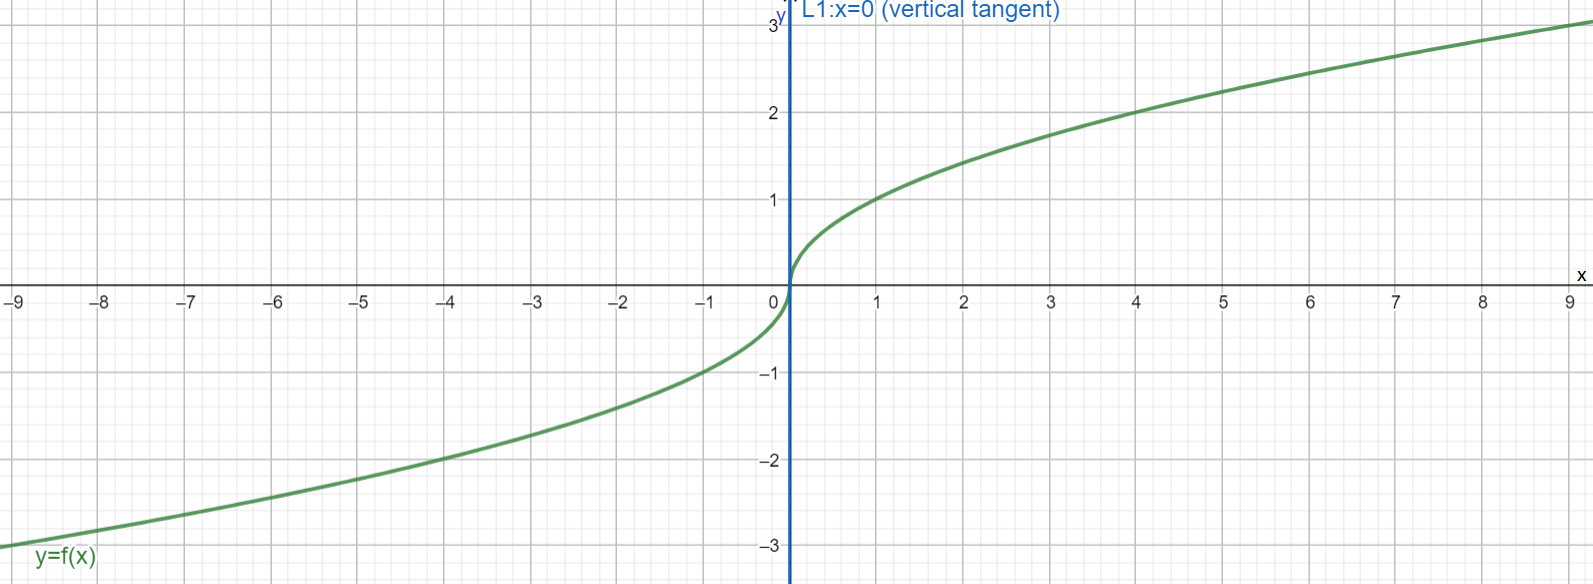
\includegraphics[scale=0.4]{img/20211117_calculusA_HW5_Fig_1.PNG}
\item \begin{enumerate}[label=(\roman*)]
    \item 
    \[\lim_{\Delta x\to 0^-} \frac{y\vert _{x=\Delta x}-y\vert _{x=0}}{\Delta x}=\lim_{\Delta x\to 0^-} \frac{-\sqrt{|\Delta x|}}{\Delta x}=\lim_{\Delta x\to 0^-} \sqrt{\frac{-\Delta x}{(-\Delta x)^2}}=+\infty\]
    \item
    \[\lim_{\Delta x\to 0^+} \frac{y\vert _{x=\Delta x}-y\vert _{x=0}}{\Delta x}=\lim_{\Delta x\to 0^+} \frac{\sqrt{\Delta x}}{\Delta x}=\lim_{\Delta x\to 0^+} \sqrt{\frac{\Delta x}{(\Delta x)^2}}=+\infty\]
\end{enumerate}
(i)$\land$(ii) $\Rightarrow \lim_{\Delta x\to 0} \frac{y\vert _{x=\Delta x}-y\vert _{x=0}}{\Delta x}=+\infty\Rightarrow$ The graph has a vertical tangent at $x=0$.
\end{enumerate}
\section*{2. Additional and Advanced Exercises}
\subsection*{19.}
\textbf{Antipodal points} Is there any reason to believe that there is always a pair of antipodal (diametrically oppositve) points on Earth's equator where the temperatures are the same? Explain.
\subsection*{Solution}
Surface temperature of the Earth can be considered as a scalar field on a sphere. \newline 
Let $\Vec{r}$ and $-\Vec{r}$ to be a pair of antipodal points on the Earth, where $\Vec{0}$ is the center of earth. \newline
Define $f$ as the "directed" temperature difference between the antipodal points, i.e. $f(\Vec{r})=T(\Vec{r})-T(-\Vec{r})$, where $T(\Vec{r})$ is the surface temperature at position $\Vec{r}$.\newline
Let $d=f(\Vec{r_0})$, where $r_0$ is arbitary position on Earth. Then for its antipodal point, $f(-\Vec{r})=-d$\newline
As temperature is continuous on every position $\Vec{r}$, the range of $f$ includes positive and negative real numbers. By intermediate theorem, $\exists \Vec{r_1}$ such that $f(\Vec{r_1})=0.\blacksquare$
\subsection*{18.}
\textbf{The Dirichlet ruler function} If $x$ is a rational number, then $x$ can be written in a unique way as a quotient of integers $m/n$ where $n>0$ and $m$ and $n$ has no common factors greater than 1. (We say that such a fraction is in \textit{lowest terms}. For example, $6/4$ wirtten in lowest terms is $3/2$.) Let $f(x)$ be defined for all $x$ in the interval $[0,1]$ by
\[f(x)=\left\{\begin{array}{ll}
1/n, & \text{if }x=m/n \text{ is a rational number in lowest terms} \\
0, & \text{ if } x \text{ is irrational.}
\end{array}\right.\]
For instance, $f(0)=f(1)=1$, $f(1/2)=1/2$, $f(1/3)=f(2/3)=1/3$, $f(1/4)=f(3/4)=1/4$, and so on.
\begin{enumerate} [label=\textbf{\alph*.}]
    \item Show that $f$ is discontinuous at every rational number in $[0,1]$.
    \item Show that $f$ is continuous at every irrational number in $[0,1]$. (Hint: If $\epsilon$ is a given positve number, show that there are only finitely many rational numbes $r$ in $[0,1]$ such that $f(r)\geq \epsilon$.)
    \item Sketch the graph of $f$. Why do you think $f$ is called the "ruler function"?
\end{enumerate}
\subsection*{Solution}
\begin{enumerate} [label=\textbf{\alph*.}]
    \item Proof:\newline
    Assume $\exists q\in \mathbb{Q}$ such that $f$ is continuous at $x=q$. Let $q=m/n$. Then 
    \[(\forall \epsilon>0)(\exists \delta>0)(|x-q|<\delta \rightarrow |f(x)-f(q)|<\epsilon)\]
    Choose $\epsilon=1/(2n)$, and $x$ be a irrational number in the $\delta-$neighborhood of $q$. Then,
    \[|f(x)-f(q)|=|\frac{1}{n}|>\frac{1}{2n}=\epsilon\]
    Hence such $q$ does not exist.\newline $\blacksquare$
    \item Proof: \newline
    Let $x\in \mathbb{R}-\mathbb{Q}$. \newline
    $(\forall \epsilon>0)(\exists N\in\mathbb{N}^*)(\frac{1}{N}<\epsilon)$. \newline
    Let $M=\{q\in \mathbb{Q}: f(q)>\epsilon\}$, where $N$ is the smallest positive integer such that $\frac{1}{N}<\epsilon$ 
     \[|M|=1+\sum _{i=2}^N \varphi(i),\] where $\varphi(n)$ is Euler's totient function.(number of positive integers less than n and coprime with n)\newline
    Let $q_i\in M(1\leq i \leq |M|)$.\newline
    Let $\delta=\min \{|x-q_i|:q_i\in M\}$
    Hence, $\lnot (\exists q\in \mathbb{Q})(|x-q|<\delta \land |f(q)|\geq \epsilon)$\newline$\blacksquare$ 
    \item The graph of $f$ is shown below.\newline
    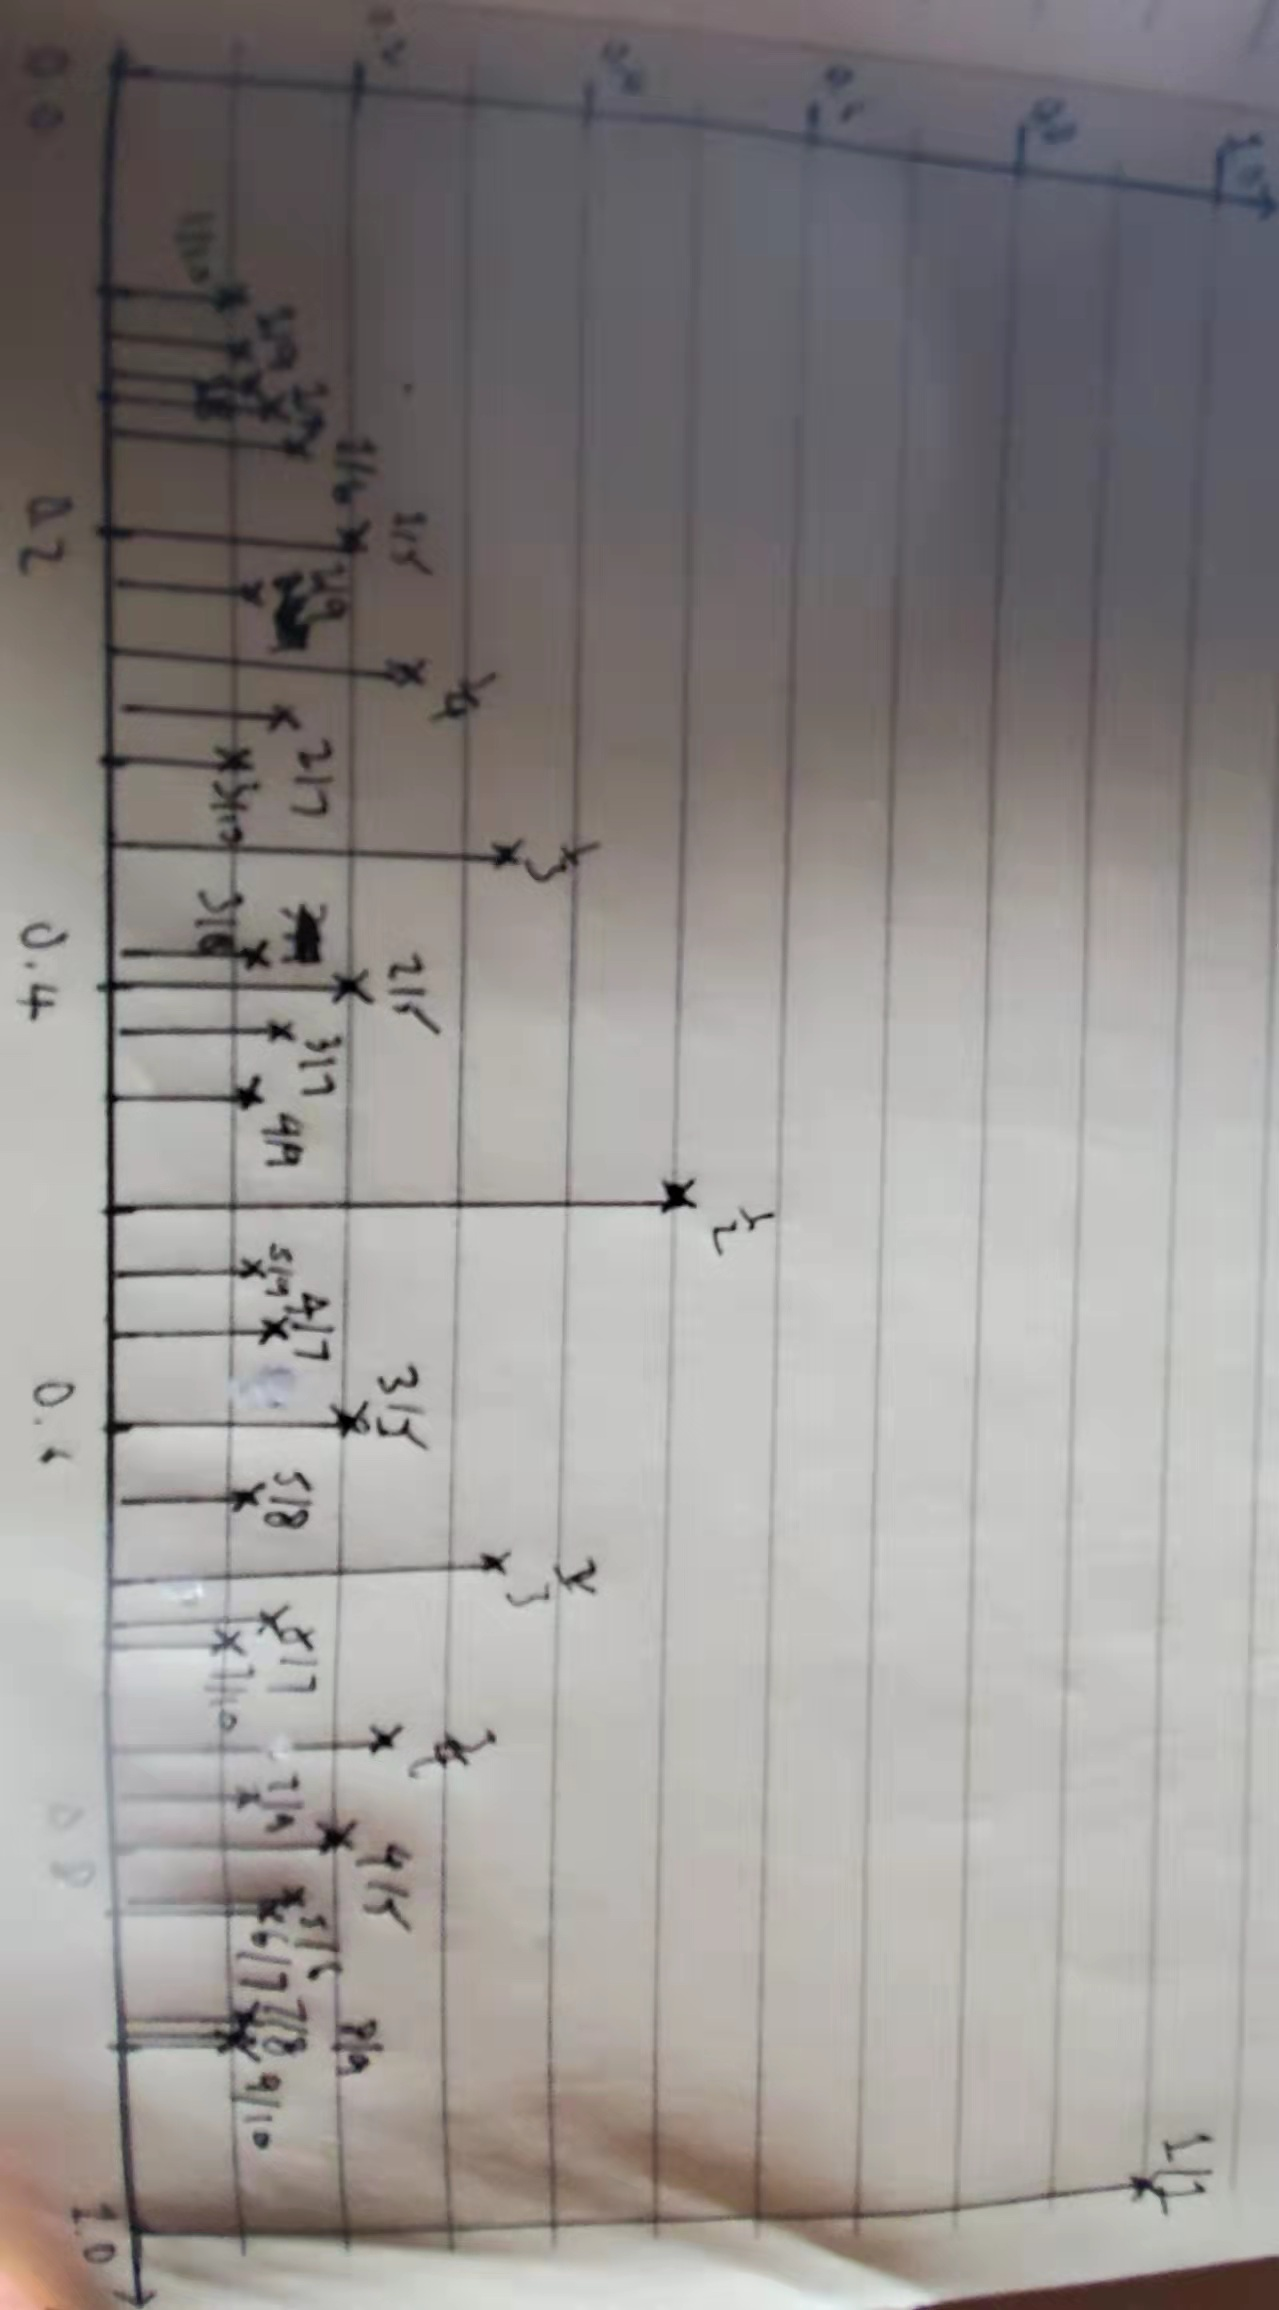
\includegraphics[width=7cm,height=14cm, angle = 90]{img/20211117_calculusA_HW5_Fig_2.PNG}\newline
    The graph looks like the markings on a ruler, when line segments with ends of $(x,0)$ and $(x,f(x))$ are constructed.
\end{enumerate}
\end{document}